%!TEX root = ../report.tex

\begin{document}
    \chapter{Experimental Setup}
    This chapter explains the model for 3D semantic segmentation, dataset trained, libraries and training parameters for Deep Ensembles and Flipout.

    \section{Semantic segmentation model}
    In this thesis, we used RandLA-Net model for 3D semantic segmentation proposed in \cite{Hu_2020_CVPR_Randla}.
    The detailed working of RandLA-Net is stated in Section~[\$].
    
    \section{Dataset}
    We use Semantic3D as our training dataset, proposed in \cite{hackel2017semantic3d}.
    The more details of the Semantic3D like dataset distribution and visual images of point cloud are represented in Section~[\$].
    We chose Semantic3D as our training set is because it being the dense dataset.
    \cite{}-[\$] states that Semantic3D is one of the dataset with low intra class variability among 3D datasets.
    That is the number of points among all the classes are nearly equal.
    Semantic3D dataset also one of the few datasets which comes with RGB values for each point.
    This helps us in understanding how important is color information in OOD detection.
    Semantic3D is an ongoing benchmark challenge, so we evaluated our trained on the valdation set.
    For a sanity check, we cross checked the performance of our trained models on this validation set with the pretrained model from authors provided in \footnote[1]{https://github.com/QingyongHu/RandLA-Net}.

    \section{Training parameters}
    In this section, we will discuss the libraries used and training parameters of the RandLA-Net for Deep Ensembles, Flipout.
    As the training and testing of Deep Neural Networks are time and resourse intensive.
    We used the High Performance Computing (HPC) GPU cluster from DFKI, especially on Nvidia Titan-XP and Nvidia-Tesla V100.
    \subsection*{Libraries}
    With the purpose of reproducibility in mind, here we provide the list of major libraries used and along with their versions, they are used for training.
    For ease of reprduction, we also added the requirements.txt in the attached code as it is a struggle to setup the environment.
    \begin{enumerate}
        \item Python - 3.6
        \item Tensorflow - 1.15.0
        \item Tensorflow probability - 0.7.0
        \item Open3d-python - 0.3.0 (training), 0.13.0 (visualizations)
    \end{enumerate}
    
    \section{RandLA-Net - Deep Ensembles}
    For Deep Ensembles, we trained 20 randomly initalized instances of RandLA-Net on Semantic3D dataset.
    We used the default training parameters provided by the authors, they are learning rate of 0.01 with decay of 0.95 multiplied for every epoch, batch size of 4 and trained for 100 epochs.
    We changed the pipeline to infer the whole point cloud and save the probability scores from these 20 models.
    These saved probabilities are them averaged and Maximum Softmax Probability (MSP) and Entropy are then extracted.
    Out of these 20 models, we provide the evaluation for every $5^{th}$ model i.e., 1, 5, 10, 15 and 20.
    \section{RandLA-Net - Flipout}
    For Flipout versioned RandLA-Net, we replaced the last three classification layers of the RandLA-Net highlighted with red box in Figure~\ref{fig:fout_randlanet} with their flipout counter parts from Tensorflow Probability.
    In addition to this change, we also removed the Dropout layer after the second classification layer.
    We chose these three layers because they are major decision makers for classification and the remaining network is a feature extraction module.
    By following the same training procedure stated by the authors, we observe similar performance so we decided not to change any training parameters.
    However, we intialized the Flipout weight perturbations with a normal prior of standard deviation 1.
    We also tried with various standard deviations such as 0.1, 0.5, 1, 1.5, 2.0 and found that standard deviation values of 0.5, 1.0 results better convergence.
    In comparison to Deep Ensembles, we performed 20 forward passes for the Flipout versioned RandLA-Net model, then averaged the results and represented every $5^{th}$ forward pass.
    \begin{figure}
        \centering
        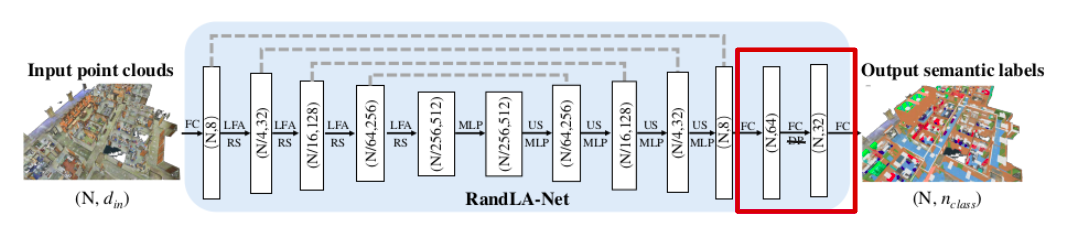
\includegraphics[scale=0.42]{images/fout_randlanet.png}
        \caption{Flipout versioned RandLA-Net where the last three FC layers are made Flipout compatible and Dropout layer represented in figure as DP strikedout.}
        \label{fig:fout_randlanet}
    \end{figure}

    \section{Summary}
    The dropout version of RandLA-Net setup is described in Section~\ref{sec:randladout} as it is only used for evaluation of OOD detection more as a baseline method.
\end{document}
